\section{Code Examples}

\begin{frame}{Sorting}
    \begin{columns}
    \column{0.7\textwidth}
        \begin{itemize}
            \item percentageFullMatch = Percentage Full Match
            \item percentagePartialMatch = Percentage Partial Match
            \item getRating = Rating
            \item prevIngredients = Previous Ingredients
            \item recipe.Title = Recipe Title
        \end{itemize}
    \column{0.3\textwidth}
        \begin{figure}
            \centering
            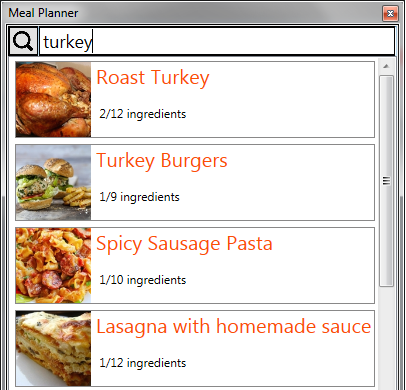
\includegraphics[width=\textwidth]{graphics/recipe-search-item}
        \end{figure}
    \end{columns}

\end{frame}

\begin{frame}[fragile]
\frametitle{PublicQuerys}
\framesubtitle{inventoryIQueryable}
\fontsize{8pt}{7}\selectfont
\begin{lstlisting}{style=cSharp}
from ii in App.db.InventoryIngredients
join i in App.db.Ingredients on ii.IngredientID equals i.ID
where ii.UserID == App.CurrentUser.ID
group ii by ii.IngredientID into iig
select new inventoryListGroupedByQuantity()
{
    IngredientID = iig.FirstOrDefault().IngredientID,
    Unit = iig.FirstOrDefault().Ingredient.Unit,
    Quantity = iig.Sum(i => i.Quantity),
    Ingredient = iig.FirstOrDefault().Ingredient,
    ExpirationDate = iig.FirstOrDefault().ExpirationDate,
    PurchaseDate = iig.FirstOrDefault().PurchaseDate,
    User = iig.FirstOrDefault().User,
    UserID = iig.FirstOrDefault().UserID
};
\end{lstlisting}
\end{frame}

\begin{frame}[fragile]
\frametitle{PublicQuerys}
\framesubtitle{inventoryList}
\fontsize{8pt}{7}\selectfont
\begin{lstlisting}{style=cSharp}
(from ii in App.db.InventoryIngredients
join i in App.db.Ingredients on ii.IngredientID equals i.ID
where ii.UserID == App.CurrentUser.ID
group ii by ii.IngredientID into iig
select new inventoryListGroupedByQuantity()
{
    IngredientID = iig.FirstOrDefault().IngredientID,
    Unit = iig.FirstOrDefault().Ingredient.Unit,
    Quantity = iig.Sum(i => i.Quantity),
    Ingredient = iig.FirstOrDefault().Ingredient,
    ExpirationDate = iig.FirstOrDefault().ExpirationDate,
    PurchaseDate = iig.FirstOrDefault().PurchaseDate,
    User = iig.FirstOrDefault().User,
    UserID = iig.FirstOrDefault().UserID
}).ToList();
\end{lstlisting}
\end{frame}

\begin{frame}[fragile]
\frametitle{PublicQuerys}
\framesubtitle{ingredientsFromLastMeals}
\fontsize{8pt}{7}\selectfont
\begin{lstlisting}{style=cSharp}
(from meals in App.db.Meals
join ri in App.db.RecipeIngredients on meals.RecipeID equals ri.RecipeID
join i in App.db.Ingredients on ri.IngredientID equals i.ID
where meals.UserID == App.CurrentUser.ID && meals.Date <= DateTime.Now
group i by i.ID into igrouped
select new LastMeal()
{
    ingredientID = igrouped.FirstOrDefault().ID,
    ingredientCount = igrouped.Count()
}).ToList();
\end{lstlisting}
\end{frame}

\begin{frame}[fragile]
\frametitle{PublicQuerys}
\framesubtitle{blackList}
\fontsize{8pt}{7}\selectfont
\begin{lstlisting}{style=cSharp}
(from bl in App.db.BlacklistIngredients
join ri in App.db.RecipeIngredients on bl.IngredientID equals ri.IngredientID
where bl.UserID == App.CurrentUser.ID
group ri by ri.RecipeID into ri
select ri.FirstOrDefault().RecipeID).ToList();
\end{lstlisting}
\end{frame}

\begin{frame}[fragile]
\frametitle{PublicQuerys}
\framesubtitle{grayList}
\fontsize{8pt}{7}\selectfont
\begin{lstlisting}{style=cSharp}
(from gl in App.db.GraylistIngredients
join i in App.db.Ingredients on gl.IngredientID equals i.ID
where gl.UserID == App.CurrentUser.ID
group gl by gl.IngredientID into gl
select new GrayList()
{
    ingredient = gl.FirstOrDefault().Ingredient,
    rating = (gl.Sum(r => r.IngredientValue) / gl.Count())
}).ToList();
\end{lstlisting}
\end{frame}







\begin{frame}{Search by recipes}
    \begin{figure}
        \centering
        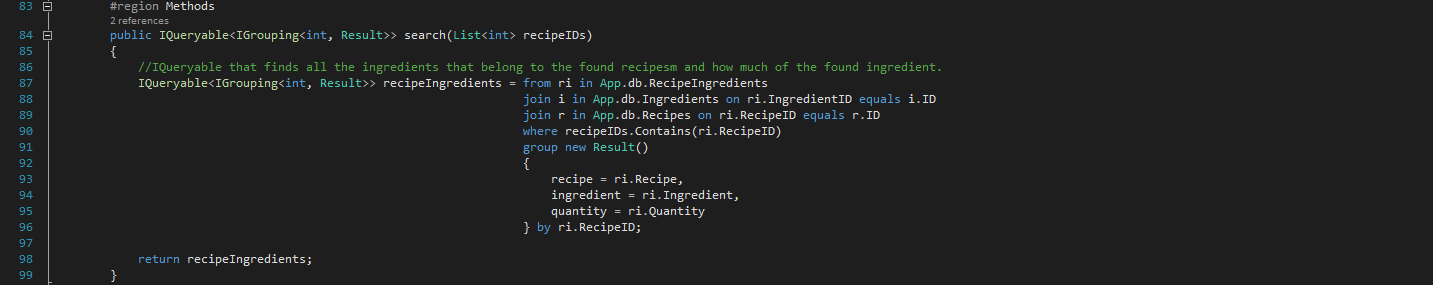
\includegraphics[width=\textwidth]{Grafik/search}
    \end{figure}
\end{frame}

\begin{frame}{Sorting of results}
    \begin{figure}
        \centering
        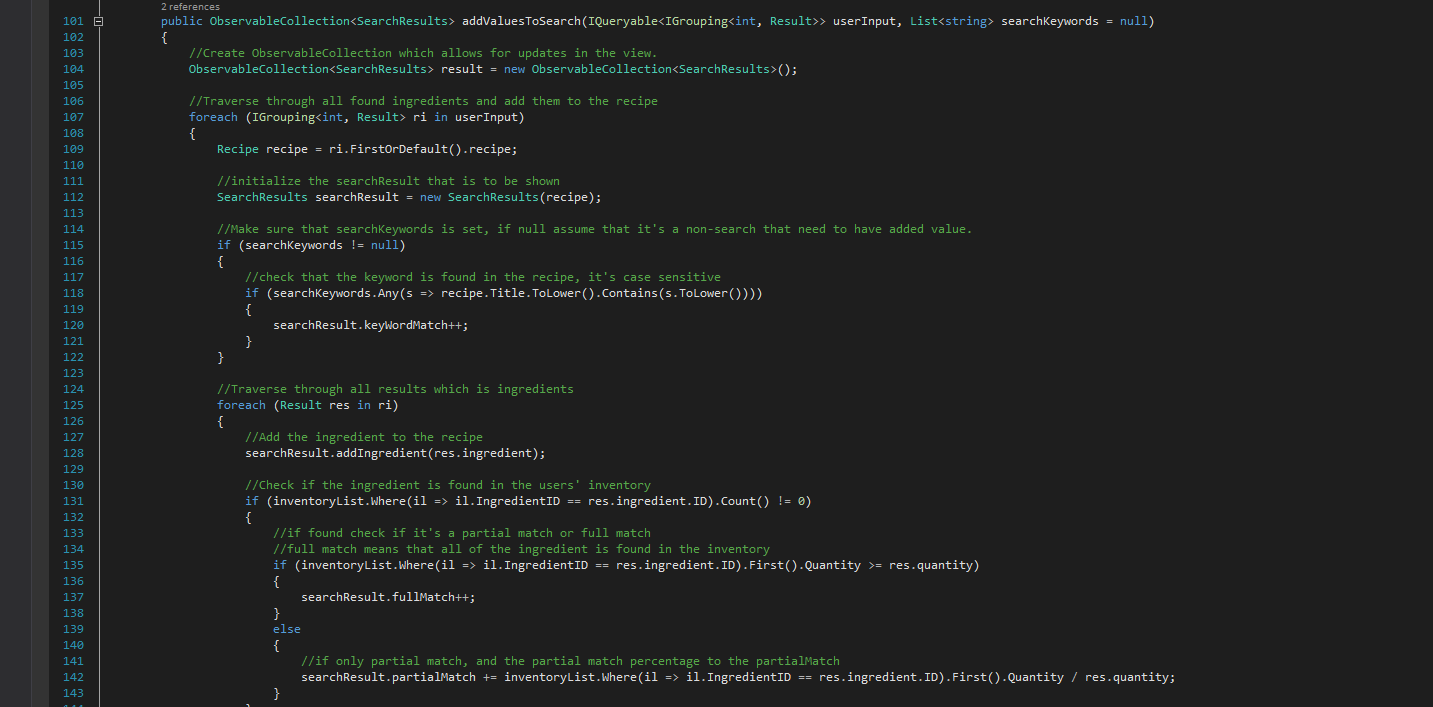
\includegraphics[width=\textwidth]{Grafik/sorter1}
    \end{figure}
\end{frame}
\begin{frame}{Sorting of results}
    \begin{figure}
        \centering
        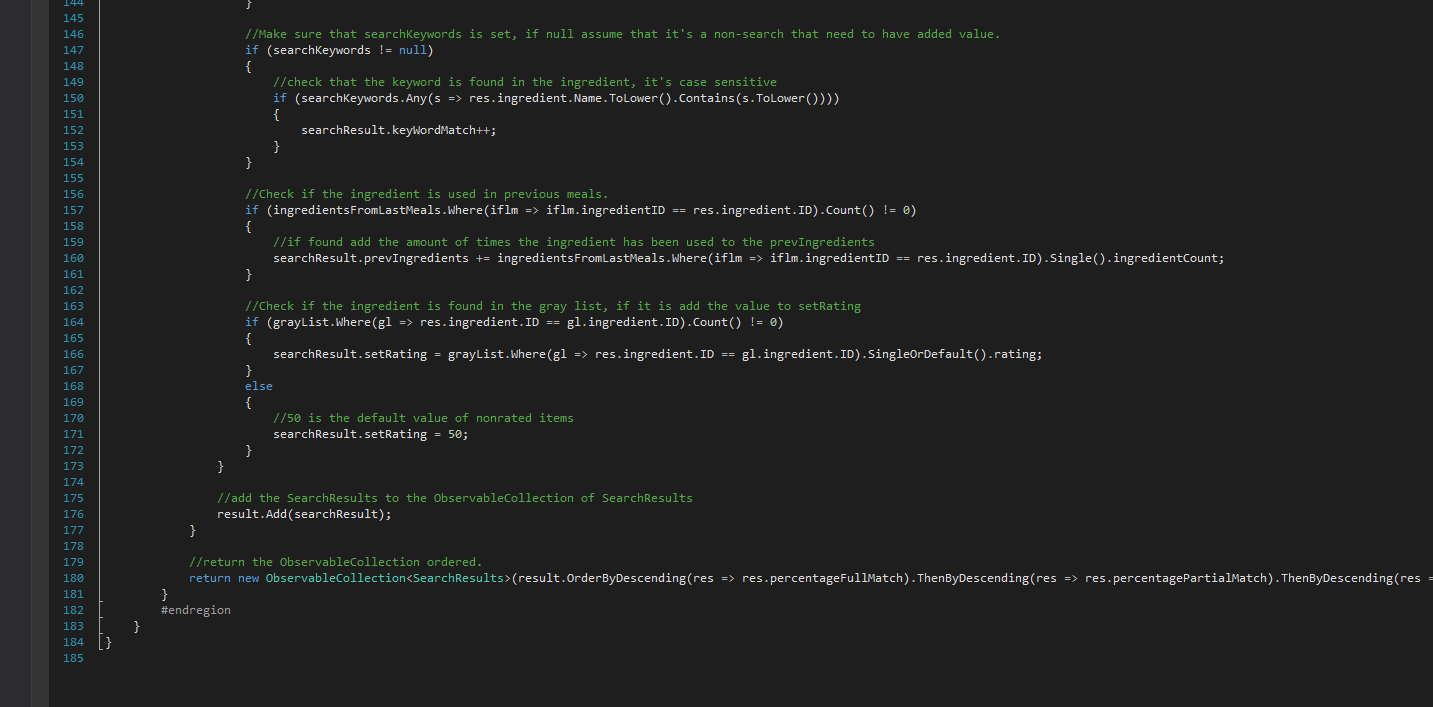
\includegraphics[width=\textwidth]{Grafik/sorter2}
    \end{figure}
\end{frame}




















